% ---------------------------------------------------------------- 23 Nov 2026: how the cavern-rock x mu pairs form (4-station + TD good track, preliminary)
\begin{btframe}{7 · Back-up · cavern-rock × μ pairs}{Cavern-rock × μ pairs: where the vertex is and which particles (4 stations + TD, preliminary)}
\noindent \begin{minipage}[t]{\dimexpr(0.50\linewidth-0.50\dimexpr9.67pt\relax)}\vspace{0pt}\centering
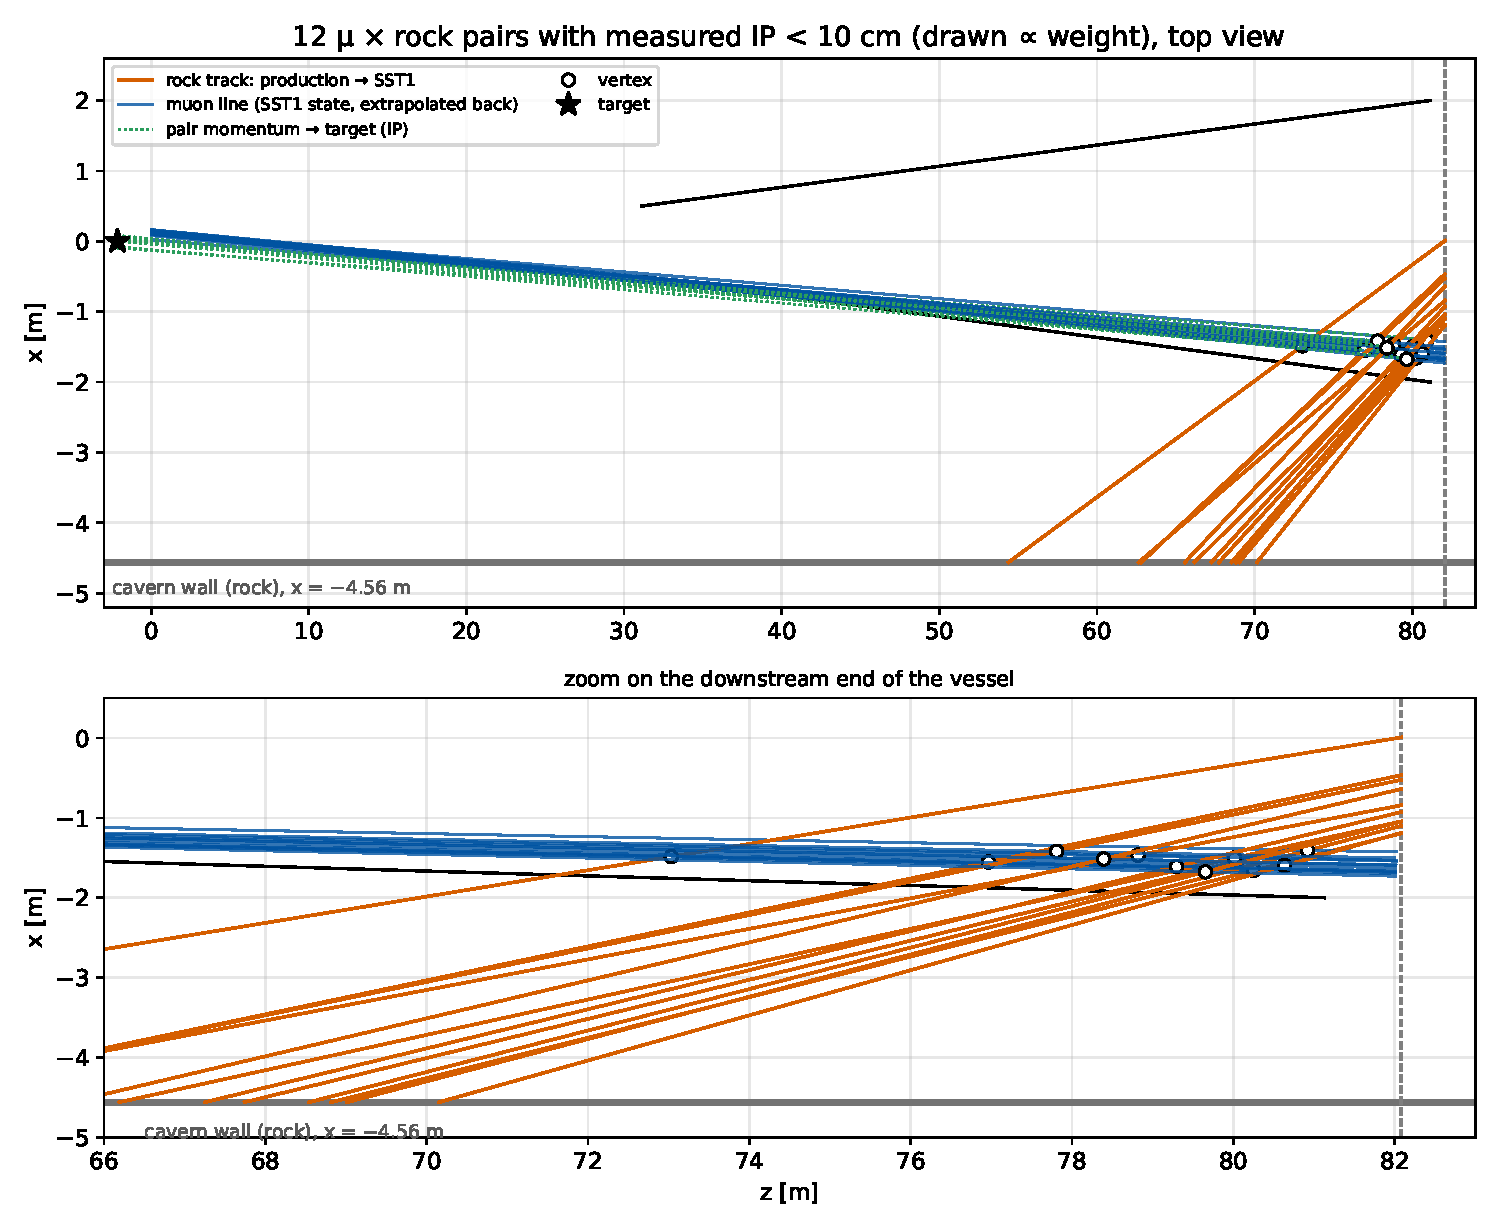
\includegraphics[width=\linewidth,height=165pt,keepaspectratio]{figs/s47_rock_mu_pairs.pdf}\par
\end{minipage}%
\hfill%
\begin{minipage}[t]{\dimexpr(0.50\linewidth-0.50\dimexpr9.67pt\relax)}\vspace{0pt}\raggedright
\begin{itemize}
  \item \textbf{Rock leg:} soft negative hadron (median 1.8 GeV) from the −x cavern wall at z ≈ 59–69 m, entering the vessel through the −x wall
  \item \textbf{Muon leg:} hard μ\textsuperscript{+} (median 218 GeV) along the −x wall; alone it misses the target by +18 cm
  \item \textbf{Vertex:} large opening angle (219 mrad) → closest approach just inside the −x wall, z ≈ 77–81 m; the rock leg tilts the pair onto the target (+3 cm)
\end{itemize}
\vspace{2pt}
{\fontsize{5.02pt}{6.52pt}\selectfont\setlength{\tabcolsep}{3.2pt}\renewcommand{\arraystretch}{1.42}
\begin{tabularx}{\linewidth}{>{\raggedright\arraybackslash}Xrrrr}
\textcolor{muted}{pairs / 15 y, before tagging (PDG μ, rock)} & \textcolor{muted}{w\textsubscript{μ} / spill} & \textcolor{muted}{w\textsubscript{rock} / spill} & \textcolor{muted}{IP < 10 cm} & \textcolor{muted}{share} \\\headrule
μ\textsuperscript{+} × π\textsuperscript{−} (−13, −211) & 0.17 & 4.6 & 62 & 74 \% \\\rowrule
μ\textsuperscript{+} × K\textsuperscript{−} (−13, −321) & 0.17 & 4.5 & 11.5 & 14 \% \\\rowrule
μ\textsuperscript{+} × p̄ (−13, −2212) & 0.17 & 4.4 & 6.1 & 7 \% \\\rowrule
μ\textsuperscript{+} × e\textsuperscript{−} (−13, 11) & 0.17 & 4.9 & 3.8 & 5 \% \\\rowrule
μ\textsuperscript{−} × positive (13, +) & 0.002–0.12 & 4.1–5.1 & < 0.02 & 0 \\\rowrule
\rowcolor{tint}\bfseries total (candidates 213, IP < 2.5 m 208) & & & \bfseries 84 & \\\rowrule
\end{tabularx}\par}
\vspace{2pt}
\begin{itemize}
  \item 4 stations + TD on both legs: 213 / 84 / 208 per 15 y (SST1 + TD: 634 / 211 / 626); weights = median per leg
  \item After tagging (SST1 + TD runs): R1 0.59, R2 / R3 < 0.018 (90 \% CL); current Z2 / Z3 and the 4-station re-run in production
\end{itemize}
\end{minipage}\par
\end{btframe}
